\begin{frame}
  \frametitle{Kerr effect: Mathematical formulation}

  With a centrosymmetric and isotropic medium the important term is
  \[
  \mathbf P = \epsilon_0 ( \chi\order1 \mathbf E +
  {\chi\order2 \mathbf E^2} + \textcolor{red}{\chi\order3 \mathbf E^3} \dots )
  \]
\end{frame}

\begin{frame}
  \frametitle{Suspectibility}

  The refractive index of the medium will then be intensity dependent. 
  \begin{align*}
    n &= \sqrt{1 + \chi_1 + \chi_3 |\mathcal{E}|^2}\\
    &\simeq n_0 + \tfrac{1}{2} n_2 |\mathcal{E}|^2,
  \end{align*}
\end{frame}

\begin{frame}
  \frametitle{Gaussion beams}
  Assume: Beam has a gaussian shape

  $\Rightarrow$ Refractive index is peaked at center.
  {\centering
  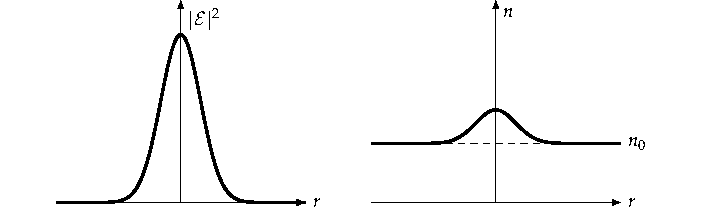
\includegraphics[width=1\columnwidth]{gaussrefrac}}

This is effectively a positive lens that will focus the beam. 
\end{frame}

\begin{frame}
  \frametitle{Waveequation}
  Assume: Monocromatic linear polarized plane wave.
  \[E = \mathcal{E}(x,y) e^{-i (\omega t-kz)}\]
  Insert into to the wave equation
\[  \nabla^2 E - \frac{1}{c^2} \ppdiff{E}{t}
  = \frac{1}{\epsilon_0c^2} \ppdiff{P}{t}\]
  This gives the nonlinear wave equation:

  \[\nabla^2 \mathcal{E} + \frac{\omega^{2}}{c^2} \mathcal{E} = - \frac{\omega^2}{\epsilon_0 c^2} \left( \epsilon_0 \chi_1
    \mathcal{E} + \epsilon_0 \chi_3 |\mathcal{E}|^2 \mathcal{E}
  \right).\]

  which is a partial differential equation !
\end{frame}


%%% Local Variables: 
%%% mode: latex
%%% TeX-master: "nonlinearslides"
%%% End: 
